\documentclass[12pt,a4paper]{article}

% ===== GÓI CẦN THIẾT =====
\usepackage[utf8]{vietnam}
\usepackage{graphicx}
\usepackage{geometry}
\usepackage{setspace}
\usepackage{fancyhdr}
\usepackage{tikz}
\usepackage{hyperref}
\usepackage{booktabs}
\usepackage{array}
\usepackage{xcolor}
\usepackage{listings}
\usepackage{tocloft}
\usepackage{float}

\geometry{top=2.5cm,bottom=2.5cm,left=3cm,right=2.5cm}
\onehalfspacing
\fontsize{11pt}{12.5pt}\selectfont

% ===== KHUNG TRANG =====
\newcommand{\pageborder}{
\begin{tikzpicture}[remember picture,overlay]
  \draw[line width=1pt]
    ($(current page.north west)+(1.5cm,-1.5cm)$)
    rectangle
    ($(current page.south east)+(-1.5cm,1.5cm)$);
\end{tikzpicture}
}

% ===== CẤU HÌNH HEADER/FOOTER =====
\pagestyle{fancy}
\fancyhf{}
\fancyhead[R]{\small Báo cáo GR1 - Hệ thống quản lý ký túc xá}
\fancyfoot[C]{\thepage}
\renewcommand{\headrulewidth}{0.5pt}

% ===== CẤU HÌNH CODE =====
\lstset{
  basicstyle=\ttfamily\small,
  breaklines=true,
  frame=single,
  language=JavaScript,
  commentstyle=\color{gray},
  keywordstyle=\color{blue},
  stringstyle=\color{red},
  showstringspaces=false
}

\begin{document}

% ===== TRANG BÌA =====
\pageborder
\thispagestyle{empty}

\begin{center}

\textbf{\Large ĐẠI HỌC BÁCH KHOA HÀ NỘI}\\[0.3cm]
\textbf{TRƯỜNG CÔNG NGHỆ THÔNG TIN VÀ TRUYỀN THÔNG}\\[1.5cm]

\textbf{\Large BÁO CÁO NGHIÊN CỨU TỐT NGHIỆP 2}\\[1cm]

\textbf{\LARGE HỆ THỐNG QUẢN LÝ KÝ TÚC XÁ}\\[0.3cm]
\textbf{\LARGE CHO SINH VIÊN}\\[2cm]

\begin{flushleft}
\hspace{3cm}Giảng viên hướng dẫn: \textbf{PGS.TS. Cao Tuấn Dũng}\\[0.5cm]
\hspace{3cm}Sinh viên thực hiện: \textbf{Phan Đức Quyền}\\[0.5cm]
\hspace{3cm}Mã số sinh viên: \textbf{20225916}\\[0.5cm]
\hspace{3cm}Lớp: \textbf{ATTT-K68}\\[2cm]
\end{flushleft}

\vfill

\textbf{Hà Nội, tháng 1 năm 2026}

\end{center}

% ===== TRANG MỤC LỤC =====
\newpage
\pagestyle{empty}
\tableofcontents
\newpage

% ===== DANH SÁCH HÌNH =====
\listoffigures
\newpage

% ===== DANH SÁCH BẢNG =====
\listoftables
\newpage

\pagestyle{fancy}

% ===== PHẦN 1: GIỚI THIỆU ĐỀ TÀI =====
\section{GIỚI THIỆU ĐỀ TÀI}

\subsection{Đặt vấn đề}

Trong bối cảnh phát triển mạnh mẽ của công nghệ thông tin và xu hướng số hóa các hoạt động quản lý, việc xây dựng một hệ thống quản lý ký túc xá hiện đại trở nên cấp thiết và cần thiết. Hiện tại, tại Đại học Bách Khoa Hà Nội, quy trình quản lý ký túc xá còn nhiều hạn chế:

\begin{itemize}
  \item Quy trình thủ công: Việc đăng ký phòng, quản lý thông tin sinh viên chủ yếu dùng giấy tờ hoặc Excel
  \item Thiếu tính minh bạch: Sinh viên khó tra cứu thông tin phòng trống, tiến độ xét duyệt
  \item Khó khăn trong quản lý: Cán bộ gặp khó khăn theo dõi tổng thể tình trạng lấp đầy
  \item Thiếu tích hợp: Thông tin rải rác, không có hệ thống tổng thể
\end{itemize}

\subsection{Mục tiêu, phạm vi và ý nghĩa}

\textbf{Mục tiêu:} (1) Xây dựng hệ thống web quản lý ký túc xá với chức năng đăng ký phòng, quản lý sinh viên, thống kê báo cáo; (2) Ứng dụng công nghệ web hiện đại (Node.js, Express.js, MongoDB); (3) Nâng cao hiệu quả quản lý, tính minh bạch thông tin.

\textbf{Phạm vi:} Hệ thống phục vụ Đại học Bách Khoa Hà Nội, đối tượng: sinh viên và cán bộ quản lý. Module sinh viên (đăng ký phòng, xem thông tin, yêu cầu ưu tiên), module quản trị (CRUD ký túc xá/phòng, xét duyệt đơn, phân phòng tự động). Công nghệ: Frontend (EJS, Bootstrap, Leaflet), Backend (Node.js, Express), Database (MongoDB, Mongoose), Bảo mật (Bcrypt, 2FA).

\textbf{Ý nghĩa:} Số hóa quy trình quản lý thủ công, cải thiện dịch vụ, giảm tải cán bộ, tạo nền tảng mở rộng.

% ===== PHẦN 2: KHẢO SÁT VÀ PHÂN TÍCH YÊU CẦU =====
\newpage
\section{KHẢO SÁT VÀ PHÂN TÍCH YÊU CẦU}

\subsection{Khảo sát nền tảng và yêu cầu}

Các nền tảng quốc tế (Scape.com.au, University Living) cung cấp: giao diện responsive, tìm kiếm/lọc nâng cao, bản đồ tương tác, thông báo real-time, hệ thống đánh giá. Quy trình: (1) Tìm kiếm, (2) Xem chi tiết, (3) Điền thông tin, (4) Thanh toán, (5) Xác nhận qua email/SMS.

\subsection{Yêu cầu hệ thống}

\textbf{Chức năng sinh viên:} Đăng ký, xác thực 2FA, xem danh sách ký túc xá, đăng ký phòng, theo dõi đơn, xem bản đồ, yêu cầu ưu tiên.

\textbf{Chức năng admin:} CRUD ký túc xá/phòng, xét duyệt đơn, phân phòng tự động, báo cáo thống kê, thông báo hệ thống.

\begin{table}[h]
\centering
\fontsize{10pt}{11pt}\selectfont
\caption{Yêu cầu phi chức năng}
\begin{tabular}{|l|l|}
\hline
\textbf{Tiêu chí} & \textbf{Chi tiết} \\
\hline
Hiệu suất & Response < 2 giây \\
Bảo mật & Bcrypt, 2FA, SSL/TLS \\
Khả năng mở rộng & Hỗ trợ 10,000+ người dùng \\
Độ tin cậy & Backup tự động \\
\hline
\end{tabular}
\end{table}

% ===== PHẦN 3: CÔNG NGHỆ SỬ DỤNG =====
\newpage
\section{CÔNG NGHỆ SỬ DỤNG VÀ PHÂN TÍCH KỸ THUẬT}

\subsection{Kiến trúc hệ thống}

Hệ thống được thiết kế theo mô hình 3-tiers: (1) \textbf{Presentation Layer} - Frontend với EJS, HTML5, CSS3, JavaScript; (2) \textbf{Business Logic Layer} - Backend với Node.js, Express.js; (3) \textbf{Data Access Layer} - MongoDB với Mongoose ODM.

\subsection{Công nghệ Frontend}

\textbf{EJS Template Engine:} Embedded JavaScript cho phép tạo HTML động phía server, tích hợp dễ dàng với Express.js, hỗ trợ template inheritance.

\textbf{HTML5/CSS3 Responsive:} Semantic markup, flexbox layout, grid system, mobile-first design. CSS3 hỗ trợ gradient, animation, transition.

\textbf{JavaScript ES6+:} Arrow functions, template literals, async/await, destructuring, classes cho việc quản lý DOM và gọi API.

\textbf{Bootstrap Framework:} Grid 12-column, pre-built components (buttons, modals, forms), consistent styling, mobile optimization.

\textbf{Leaflet.js:} Thư viện bản đồ mã nguồn mở, tích hợp OpenStreetMap, hỗ trợ markers, popups, zoom, pan.

\begin{figure}[H]
\centering
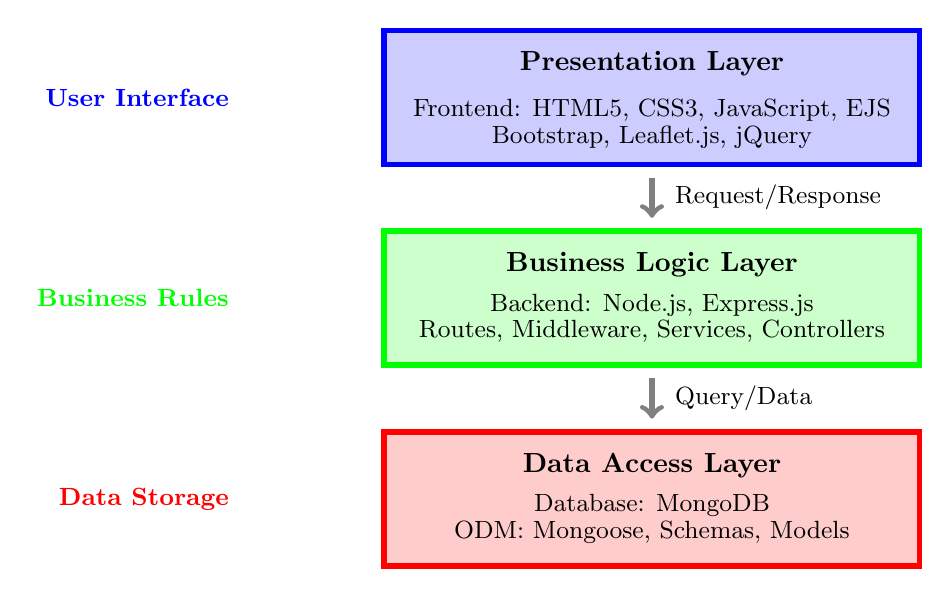
\begin{tikzpicture}[scale=0.85]
  % Presentation Layer
  \draw[fill=blue!20, draw=blue, line width=2pt] (1,8) rectangle (9,10);
  \node[font=\bfseries, align=center] at (5,9.5) {Presentation Layer};
  \node[font=\small, align=center] at (5,8.8) {Frontend: HTML5, CSS3, JavaScript, EJS};
  \node[font=\small, align=center] at (5,8.4) {Bootstrap, Leaflet.js, jQuery};
  
  % Arrow
  \draw[->, line width=2pt, gray] (5,7.8) -- (5,7.2);
  \node[right, font=\small] at (5.2,7.5) {Request/Response};
  
  % Business Logic Layer
  \draw[fill=green!20, draw=green, line width=2pt] (1,5) rectangle (9,7);
  \node[font=\bfseries, align=center] at (5,6.5) {Business Logic Layer};
  \node[font=\small, align=center] at (5,5.9) {Backend: Node.js, Express.js};
  \node[font=\small, align=center] at (5,5.5) {Routes, Middleware, Services, Controllers};
  
  % Arrow
  \draw[->, line width=2pt, gray] (5,4.8) -- (5,4.2);
  \node[right, font=\small] at (5.2,4.5) {Query/Data};
  
  % Data Access Layer
  \draw[fill=red!20, draw=red, line width=2pt] (1,2) rectangle (9,4);
  \node[font=\bfseries, align=center] at (5,3.5) {Data Access Layer};
  \node[font=\small, align=center] at (5,2.9) {Database: MongoDB};
  \node[font=\small, align=center] at (5,2.5) {ODM: Mongoose, Schemas, Models};
  
  % Side annotations
  \node[left=1cm, font=\small\bfseries, color=blue] at (0,9) {User Interface};
  \node[left=1cm, font=\small\bfseries, color=green] at (0,6) {Business Rules};
  \node[left=1cm, font=\small\bfseries, color=red] at (0,3) {Data Storage};
  
\end{tikzpicture}
\caption{Kiến trúc 3-tiers của hệ thống}
\end{figure}

\subsection{Công nghệ Backend}

\textbf{Node.js:} Runtime JavaScript trên server, event-driven non-blocking I/O, npm package manager phong phú, hiệu suất cao.

\textbf{Express.js:} Web framework minimalit, routing linh hoạt, middleware architecture, RESTful API support, session management.

\textbf{Middleware chính:}
\begin{itemize}
  \item express-session - Quản lý session người dùng với MongoDB store
  \item bcryptjs - Hash mật khẩu an toàn với salt ngẫu nhiên
  \item nodemailer - Gửi email OTP và thông báo
  \item multer - Upload file từ client
  \item cors - Cross-Origin Resource Sharing
\end{itemize}

\subsection{Công nghệ Database}

\textbf{MongoDB:} NoSQL document database, schema-less, horizontal scalability, indexing và aggregation pipeline.

\textbf{Mongoose ODM:} Object Document Mapper cho MongoDB, schema validation, pre/post hooks, population relationships.

\textbf{Collections chính:} users, dormitories, rooms, allocationCycles, registrations, priorityClaims, maintenanceRequests, violations, allocations, notifications, academicPolicies, auditLogs.

\begin{figure}[H]
\centering
\begin{tikzpicture}[scale=0.75, node distance=2cm]
  % Styles
  \tikzstyle{collection}=[rectangle, draw=blue, fill=blue!10, minimum width=2.5cm, minimum height=1.2cm, align=center, font=\small]
  \tikzstyle{arrow}=[draw=gray, ->, line width=1.5pt]
  
  % Collections
  \node[collection] (users) at (0,8) {Users};
  \node[collection] (dorms) at (5,8) {Dormitories};
  \node[collection] (rooms) at (10,8) {Rooms};
  
  \node[collection] (alloc) at (2,4) {Allocations};
  \node[collection] (cycles) at (7,4) {AllocationCycles};
  \node[collection] (regs) at (12,4) {Registrations};
  
  \node[collection] (claims) at (1,0) {PriorityClaims};
  \node[collection] (maint) at (6,0) {MaintenanceRequests};
  \node[collection] (violations) at (11,0) {Violations};
  
  % Relationships
  \draw[arrow] (users) -- (alloc);
  \draw[arrow] (dorms) -- (rooms);
  \draw[arrow] (rooms) -- (alloc);
  \draw[arrow] (cycles) -- (alloc);
  \draw[arrow] (users) -- (regs);
  \draw[arrow] (dorms) -- (regs);
  \draw[arrow] (users) -- (claims);
  \draw[arrow] (dorms) -- (claims);
  \draw[arrow] (users) -- (maint);
  \draw[arrow] (rooms) -- (maint);
  \draw[arrow] (users) -- (violations);
  \draw[arrow] (rooms) -- (violations);
  
  % Legend
  \node[right=2cm of violations, font=\small] (legend) {
    \begin{tabular}{l}
      Mũi tên: Mối quan hệ \\
      1 người dùng: nhiều đơn đăng ký \\
      1 ký túc xá: nhiều phòng \\
      1 phòng: nhiều cấp phát
    \end{tabular}
  };
  
\end{tikzpicture}
\caption{Sơ đồ mối quan hệ giữa các collection MongoDB}
\end{figure}

\subsection{Bảo mật hệ thống}

\subsubsection{Mã hóa mật khẩu với Bcryptjs}

Mật khẩu người dùng được mã hóa bằng thuật toán bcrypt, một thuật toán hashing được thiết kế đặc biệt cho mất khẩu. Hệ thống sử dụng bcryptjs với các tham số sau:

\begin{itemize}
  \item \textbf{Cost factor (salt rounds):} 10 - quy định số vòng lặp tính toán, càng cao càng an toàn nhưng chậm hơn
  \item \textbf{Salt ngẫu nhiên:} Được tạo tự động cho mỗi mật khẩu, ngăn chặn tấn công rainbow table
  \item \textbf{Output:} Hash 60 ký tự chứa salt + hash, có thể verify lại mật khẩu mà không cần lưu password gốc
\end{itemize}

Quy trình hash mật khẩu: Khi người dùng đăng ký, mật khẩu được gửi qua HTTPS → Server hash bằng bcrypt với cost factor 10 → Lưu hash vào MongoDB. Khi đăng nhập, mật khẩu nhập vào được so sánh với hash lưu trữ bằng hàm \texttt{bcrypt.compare()} mà không cần giải mã.

Ưu điểm của bcrypt: (1) Chống brute-force attack vì thời gian tính toán lâu (200ms/lần), (2) Adaptive - có thể tăng cost factor khi máy tính nhanh hơn, (3) Một mật khẩu luôn hash ra 60 ký tự khác nhau mỗi lần.

\subsubsection{Xác thực hai yếu tố (2FA) qua Email OTP}

Hệ thống áp dụng cơ chế xác thực hai yếu tố (Two-Factor Authentication) để tăng cường bảo mật tài khoản. Sau khi xác thực thành công email/mật khẩu, người dùng phải nhập mã OTP (One-Time Password) hợp lệ để hoàn tất đăng nhập.

\textbf{Quy trình xác thực 2FA:}

\begin{enumerate}
  \item Người dùng nhập email và mật khẩu trên form đăng nhập
  \item Server kiểm tra xem email/password có hợp lệ không
  \item Nếu hợp lệ, server tạo OTP 6 chữ số ngẫu nhiên
  \item OTP được lưu vào session với thời gian hiệu lực 10 phút
  \item Server gửi OTP qua email của người dùng bằng Nodemailer
  \item Người dùng nhập mã OTP vào form xác thực
  \item Server so sánh OTP nhập vào với OTP lưu trong session
  \item Nếu đúng và chưa hết thời gian, tạo session đăng nhập chính thức
  \item Người dùng được redirect tới trang dashboard
\end{enumerate}

Thông số 2FA: OTP là chuỗi 6 chữ số (000000-999999), thời gian hiệu lực 10 phút, tối đa 5 lần nhập sai trước khi phải gửi lại OTP, mỗi OTP chỉ sử dụng được 1 lần.

\subsubsection{Quản lý Session và Cookies}

Hệ thống sử dụng express-session với MongoDB store để quản lý session người dùng:

\begin{itemize}
  \item \textbf{Session Store:} Lưu trữ session vào MongoDB thay vì memory, giúp session persist qua các lần khởi động
  \item \textbf{httpOnly Cookies:} Cờ httpOnly ngăn chặn truy cập cookie từ JavaScript, chỉ gửi qua HTTP request
  \item \textbf{Secure Flag:} Cookie chỉ được gửi qua HTTPS, không gửi qua HTTP không mã hóa
  \item \textbf{SameSite Policy:} Cài đặt SameSite=Strict để chống CSRF attack
  \item \textbf{Session Timeout:} Session tự động hết hạn sau 1 giờ không hoạt động
\end{itemize}

\begin{figure}[H]
\centering
\begin{tikzpicture}[scale=0.9]
  % User (Client)
  \draw[fill=blue!20, draw=blue, line width=2pt] (0,8) rectangle (2,9);
  \node[font=\bfseries, align=center] at (1,8.5) {User\\(Browser)};
  
  % Server
  \draw[fill=green!20, draw=green, line width=2pt] (5,8) rectangle (7,9);
  \node[font=\bfseries, align=center] at (6,8.5) {Server\\(Node.js)};
  
  % Database
  \draw[fill=orange!20, draw=orange, line width=2pt] (10,8) rectangle (12,9);
  \node[font=\bfseries, align=center] at (11,8.5) {MongoDB\\(Sessions)};
  
  % Email Service
  \draw[fill=purple!20, draw=purple, line width=2pt] (10,5) rectangle (12,6);
  \node[font=\bfseries, align=center] at (11,5.5) {Email\\Service};
  
  % Step 1
  \draw[->, line width=2pt] (2,8.5) -- (5,8.5);
  \node[above, font=\small] at (3.5,8.7) {1. Email + Pass};
  
  % Step 2
  \draw[->, line width=2pt] (6,7.8) -- (6,7.2);
  \node[right, font=\small] at (6.2,7.5) {2. Verify pass};
  
  % Step 3
  \draw[->, line width=2pt, dashed] (7,8.2) -- (10,8.2);
  \node[above, font=\small] at (8.5,8.4) {3. Create session};
  
  % Step 4
  \draw[->, line width=2pt] (11,8) -- (11,6);
  \node[right, font=\small] at (11.2,7) {4. Send OTP};
  
  % Step 5
  \draw[->, line width=2pt] (11,5) -- (3,5);
  \node[below, font=\small] at (7,4.8) {5. OTP Email};
  
  % Step 6
  \draw[->, line width=2pt] (2,5) -- (5,5);
  \node[above, font=\small] at (3.5,5.2) {6. Enter OTP};
  
  % Step 7
  \draw[->, line width=2pt, dashed] (6,5) -- (11,8.2);
  \node[above, font=\small] at (8.5,6.5) {7. Verify OTP};
  
  % Step 8
  \draw[->, line width=2pt] (10,8.5) -- (7,8.5);
  \node[below, font=\small] at (8.5,8.2) {8. Session OK};
  
  % Step 9
  \draw[->, line width=2pt] (5,8.5) -- (2,8.5);
  \node[below, font=\small] at (3.5,8.2) {9. Login Success};
  
  % Legend
  \node[left, font=\small\bfseries, color=blue] at (-0.5,4) {Quy trình xác thực 2FA:};
  \node[left, font=\small] at (-0.5,3.5) {Solid: HTTP request};
  \node[left, font=\small] at (-0.5,3) {Dashed: Backend process};
  
\end{tikzpicture}
\caption{Quy trình xác thực 2FA của hệ thống}
\end{figure}

\subsubsection{Các biện pháp bảo mật bổ sung}

\textbf{HTTPS/SSL-TLS:} Tất cả giao tiếp giữa client-server được mã hóa, ngăn chặn man-in-the-middle attack.

\textbf{Input Validation:} Tất cả dữ liệu từ client đều được validate phía server, chống XSS (Cross-Site Scripting) và injection attack.

\textbf{Rate Limiting:} Giới hạn số lần đăng nhập sai để chống brute-force attack, sau 5 lần sai phải đợi 15 phút.

\textbf{CORS Policy:} Cài đặt CORS chặt chẽ, chỉ cho phép request từ domain bạn tin cậy.

\textbf{Password Policy:} Mật khẩu phải có ít nhất 8 ký tự, chứa chữ hoa, chữ thường, số và ký tự đặc biệt.

% ===== PHẦN 4: THIẾT KẾ GIAO DIỆN =====
\newpage
\section{THIẾT KẾ GIAO DIỆN HỆ THỐNG}

Hệ thống gồm ba module giao diện chính: (1) Module sinh viên, (2) Module quản trị, (3) Giao diện công khai.

\subsection{Module Sinh Viên}

\textbf{Trang Đăng Nhập/Đăng Ký:} Form đơn giản, responsive, centered layout. Sinh viên nhập email, mật khẩu, xác thực 2FA qua OTP email. Hỗ trợ quên mật khẩu, đăng ký tài khoản mới.

\textbf{Dashboard Sinh Viên:} Hiển thị thông tin cá nhân, danh sách ký túc xá khả dụng, trạng thái đơn đã đăng ký, thông báo mới nhất. Card layout, responsive.

\textbf{Danh Sách Ký Túc Xá:} Grid layout với filter sidebar. Mỗi ký túc xá hiển thị dưới dạng card chứa ảnh, tên, địa chỉ, số phòng, tỷ lệ lấp đầy, giá cả. Hỗ trợ lọc theo loại phòng, giá cả.

\textbf{Đăng Ký Phòng:} Wizard form 4 bước: (1) Chọn ký túc xá, (2) Chọn phòng, (3) Xác nhận, (4) Hoàn thành. Progress bar hướng dẫn người dùng.

\textbf{Theo Dõi Đơn:} Bảng hoặc timeline view danh sách đơn. Mỗi đơn hiển thị: ngày, ký túc xá, phòng, trạng thái (chờ/duyệt/từ chối), hành động (xem chi tiết, hủy).

\textbf{Bản Đồ Tương Tác:} Leaflet.js hiển thị bản đồ Hà Nội, markers ký túc xá, popup thông tin, tính toán khoảng cách.

\textbf{Yêu Cầu Ưu Tiên:} Form gửi yêu cầu + upload tài liệu hỗ trợ. Danh sách yêu cầu đã gửi với trạng thái xét duyệt.

\begin{figure}[H]
\centering
\includegraphics[width=10cm]{placeholder_login_form.png}
\caption{Form đăng nhập với xác thực 2FA}
\end{figure}

\begin{figure}[H]
\centering
\includegraphics[width=10.5cm]{placeholder_student_dashboard.png}
\caption{Dashboard sinh viên}
\end{figure}

\begin{figure}[H]
\centering
\includegraphics[width=10.5cm]{placeholder_dormitory_list.png}
\caption{Danh sách ký túc xá với filter}
\end{figure}

\begin{figure}[H]
\centering
\includegraphics[width=10cm]{placeholder_room_registration.png}
\caption{Form wizard đăng ký phòng}
\end{figure}

\subsection{Module Quản Trị}

\textbf{Dashboard Quản Trị:} KPI cards (tổng sinh viên, phòng trống, tỷ lệ lấp đầy), biểu đồ thống kê, danh sách đơn chờ duyệt, hoạt động gần đây.

\textbf{Quản Lý Ký Túc Xá:} CRUD tòa nhà. Bảng liệt kê với cột: tên, địa chỉ, số tầng, sức chứa, tỷ lệ lấp đầy, hành động.

\textbf{Quản Lý Phòng:} Tree view hoặc bảng (tòa → tầng → phòng). Hiển thị: số phòng, sức chứa, loại, trạng thái (màu: xanh=trống, đỏ=chiếm, xám=bảo trì), sinh viên. Hỗ trợ bulk update tình trạng.

\textbf{Xét Duyệt Đơn:} Danh sách đơn chờ duyệt. Mỗi đơn có chi tiết sinh viên, lựa chọn phòng từ danh sách phòng trống, nút phân phòng tự động/thủ công, phê duyệt/từ chối.

\textbf{Quản Lý Sinh Viên:} Bảng tất cả sinh viên với filter (tên, lớp, năm, trạng thái). Hành động: xem chi tiết, sửa, xóa, xem lịch sử.

\textbf{Quản Lý Yêu Cầu Ưu Tiên:} Danh sách yêu cầu, xem tài liệu kèm theo, phê duyệt/từ chối.

\textbf{Quản Lý Bảo Trì:} Danh sách ticket bảo trì. Trạng thái: chờ/đang xử lý/hoàn thành. Phân công kỹ thuật viên, cập nhật tiến độ.

\textbf{Quản Lý Vi Phạm:} Ghi nhận vi phạm sinh viên. Mức phạt tính tự động theo bảng phạt.

\textbf{Quản Lý Chu Kỳ:} Tạo chu kỳ đăng ký, cài đặt ngày bắt đầu/kết thúc, kích hoạt/đóng.

\textbf{Báo Cáo:} Tỷ lệ lấp đầy theo tòa/tầng, thống kê đơn, sinh viên chưa phân, lịch sử vi phạm. Export PDF/Excel.

\textbf{Gửi Thông Báo:} Soạn thông báo hệ thống, chọn đối tượng, schedule gửi, xem lịch sử.

\begin{figure}[H]
\centering
\includegraphics[width=10.5cm]{placeholder_admin_dashboard.png}
\caption{Dashboard quản trị}
\end{figure}

\begin{figure}[H]
\centering
\includegraphics[width=10cm]{placeholder_dormitory_management.png}
\caption{Quản lý ký túc xá}
\end{figure}

\begin{figure}[H]
\centering
\includegraphics[width=10.5cm]{placeholder_approve_registration.png}
\caption{Xét duyệt đơn đăng ký}
\end{figure}

\subsection{Giao Diện Công Khai}

\textbf{Trang Chủ:} Landing page chuyên nghiệp. Hero section với tiêu đề, mô tả, nút đăng nhập/đăng ký. Phía dưới là giới thiệu tính năng, lợi ích, tin tức mới nhất.

\begin{figure}[H]
\centering
\includegraphics[width=10.5cm]{placeholder_homepage.png}
\caption{Trang chủ công khai}
\end{figure}

% ===== PHẦN 5: IMPLEMENTATION =====
\newpage
\section{IMPLEMENTATION VÀ PHÁT TRIỂN CHỨC NĂNG}

\subsection{Kiến trúc Project và Xác Thực}

Cấu trúc thư mục: \texttt{src/config/} (cấu hình DB, logger), \texttt{src/middleware/} (auth, authorization), \texttt{src/routes/} (API routes), \texttt{src/schemas/} (Mongoose schemas), \texttt{src/services/} (business logic), \texttt{src/utils/} (utility functions), \texttt{views/} (EJS templates), \texttt{public/} (CSS, JS, images).

\textbf{Đăng ký tài khoản:} Validate dữ liệu → Kiểm tra email tồn tại → Hash mật khẩu bcrypt(password, 10) → Lưu DB → Gửi email xác thực.

\textbf{Đăng nhập 2FA:} Verify email/password → Tạo OTP ngẫu nhiên → Lưu vào session (thời gian 10 phút) → Gửi email OTP → Người dùng nhập OTP → Verify → Tạo session → Redirect.

\subsection{Quản Lý Chu Kỳ và Đăng Ký Phòng}

Chu kỳ có các trạng thái: PENDING → ACTIVE → CLOSED → PROCESSING → COMPLETED.

Quy trình đăng ký: Kiểm tra chu kỳ ACTIVE → Sinh viên chưa có phòng → Không có đơn chờ duyệt → Chọn tòa/phòng → Submit → Lưu AllocationRegistrations collection.

Phân phòng tự động:
\begin{itemize}
  \item Lấy danh sách đơn chờ duyệt sắp xếp FIFO
  \item Ưu tiên sinh viên có approved priority claims
  \item Cho mỗi đơn: tìm phòng trống, tạo RoomAllocation, cập nhật trạng thái phòng
  \item Gửi thông báo sinh viên
\end{itemize}

\subsection{Các Tính Năng Chính}

\textbf{Yêu Cầu Ưu Tiên:} Sinh viên gửi form + upload tài liệu → Admin xét duyệt → Nếu phê duyệt, sinh viên được ưu tiên trong phân phòng.

\textbf{Quản Lý Vi Phạm:} Admin ghi nhận vi phạm, tính mức phạt tự động theo bảng. Tích lũy phạt để xem xét cấm đăng ký lần sau.

\textbf{Yêu Cầu Bảo Trì:} Sinh viên báo sự cố phòng → Admin phân công kỹ thuật viên → Cập nhật tiến độ → Đánh dấu hoàn thành.

\textbf{Thông Báo Hệ Thống:} Tự động gửi khi: đơn duyệt/từ chối, phòng được phân, ưu tiên được xử lý, bảo trì hoàn thành. Admin có thể soạn thông báo thủ công, schedule gửi.

\subsection{Công Nghệ Triển Khai}

\textbf{Bản Đồ Leaflet:} Khởi tạo map với OpenStreetMap, thêm markers ký túc xá, popup thông tin.

\begin{lstlisting}[caption=Khởi tạo bản đồ]
const map = L.map('map')
  .setView([21.0285, 105.8542], 13);
  
dormitories.forEach(dorm => {
  L.marker([dorm.latitude, dorm.longitude])
    .bindPopup(dorm.name)
    .addTo(map);
});
\end{lstlisting}

\textbf{Báo Cáo:} Tỷ lệ lấp đầy theo tòa/tầng, thống kê đơn, sinh viên chưa phân. Export PDF/Excel sử dụng pdfkit, exceljs.

% ===== PHẦN 6: KẾT LUẬN =====
\newpage
\section{KẾT LUẬN VÀ HƯỚNG PHÁT TRIỂN}

\subsection{Những thành tựu đạt được}

Hệ thống đã hoàn thành: (1) Xây dựng hệ thống web với chức năng quản lý ký túc xá, (2) Bảo mật 2FA, (3) Giao diện responsive, (4) Phân phòng tự động/thủ công, (5) Yêu cầu ưu tiên, (6) Dashboard thống kê, (7) Bản đồ tương tác.

\subsection{Phát triển tương lai}

\textbf{Ngắn hạn:} Ứng dụng di động, thanh toán online, chatbot AI, analytics.

\textbf{Dài hạn:} Machine Learning dự đoán nhu cầu, mở rộng đa trường, IoT quản lý phòng thông minh.

\subsection{Bài học rút ra}

Thiết kế database chuẩn từ đầu, bảo mật ưu tiên hàng đầu, testing song song với phát triển, user feedback qua trọng, documentation chi tiết.

% ===== PHẦN 7: TÀI LIỆU THAM KHẢO =====
\newpage
\section{TÀI LIỆU THAM KHẢO}

\begin{enumerate}

\item Node.js Foundation. (2024). Node.js Documentation. 
  \textit{https://nodejs.org/docs/}

\item Express.js. (2024). Express Web Framework. 
  \textit{https://expressjs.com/}

\item MongoDB, Inc. (2024). MongoDB Manual. 
  \textit{https://docs.mongodb.com/manual/}

\item Mongoose Documentation. (2024). Mongoose ODM. 
  \textit{https://mongoosejs.com/}

\item Leaflet. (2024). Leaflet - Interactive Maps. 
  \textit{https://leafletjs.com/}

\item Bootstrap. (2024). Bootstrap Framework. 
  \textit{https://getbootstrap.com/}

\item npm. (2024). npm - JavaScript Package Manager. 
  \textit{https://www.npmjs.com/}

\item EJS. (2024). Embedded JavaScript Templating. 
  \textit{https://ejs.co/}

\item OWASP. (2024). Web Application Security. 
  \textit{https://owasp.org/}

\item Chart.js. (2024). Simple HTML5 Charts. 
  \textit{https://www.chartjs.org/}

\item bcryptjs. (2024). Bcrypt Password Hashing Library. 
  \textit{https://www.npmjs.com/package/bcryptjs}

\item Nodemailer. (2024). Email Sending Library. 
  \textit{https://nodemailer.com/}

\item Multer. (2024). File Upload Middleware. 
  \textit{https://www.npmjs.com/package/multer}

\item Postman. (2024). API Testing Tools. 
  \textit{https://www.postman.com/}

\item Git. (2024). Version Control System. 
  \textit{https://git-scm.com/}

\item Docker. (2024). Container Platform. 
  \textit{https://www.docker.com/}

\item PhanĐức Quyền. (2025). Hệ thống quản lý ký túc xá - GitHub Repository.
  \textit{https://github.com/QuyenPhan1/Dormitory\_Graduation}

\end{enumerate}

% ===== PHỤ LỤC =====
\newpage
\appendix
\section{CẤU HÌNH MÔI TRƯỜNG}

\textbf{Dependencies chính:} express, mongoose, bcryptjs, express-session, ejs, nodemailer, multer, dotenv.

\textbf{Biến môi trường:} MONGODB\_URI, SESSION\_SECRET, EMAIL\_USER, EMAIL\_PASS, PORT, NODE\_ENV.

\end{document}
